\renewcommand{\marginalheight}{25pt}
\newcommand{\varphiheight}{38pt}
\newcommand{\fieldheight}{48pt}
\begin{figure}[t]
\centering
    \hspace{-2em}
    \begin{tabular}{p{51pt}@{\hspace{25pt}}m{1pt}c@{\hspace{15pt}}m{1pt}c@{\hspace{15pt}}m{1pt}c}
      \raisebox{23pt}{
      \centering
      \begin{tabular}{c}
        \small$\texttt{Ising}$ \\
        \hspace{5pt}
        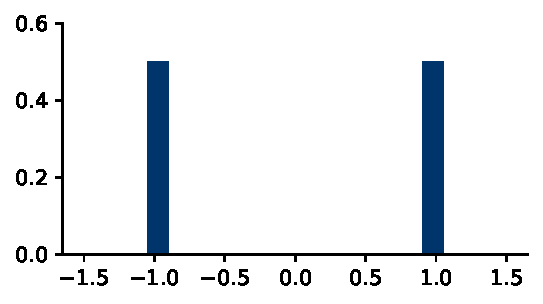
\includegraphics[height=\marginalheight]{figures/task/marginal/ising.pdf}
      \end{tabular}} &
      \raisebox{48pt}{\rotatebox{90}{\tiny $\varphi(a)$}} &
      \raisebox{8pt}{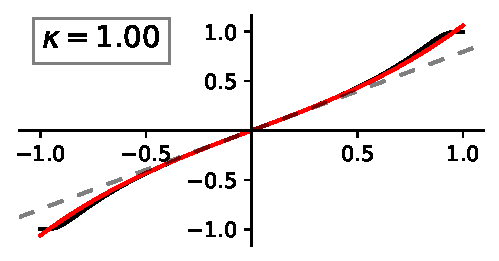
\includegraphics[height=\varphiheight]{figures/theory/varphi/ising.pdf}} & 
      \raisebox{44pt}{\rotatebox{90}{\tiny magnitude $w_i$}} &
      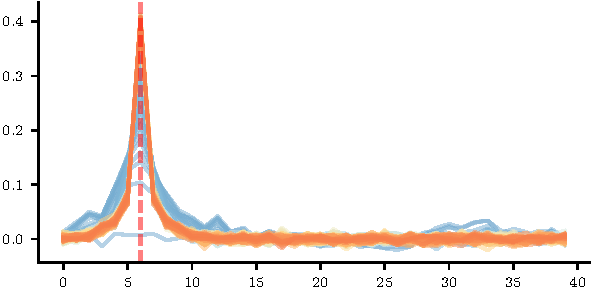
\includegraphics[height=\fieldheight]{figures/theory/rf_evol/ising_neurips.pdf} & 
      \raisebox{44pt}{\rotatebox{90}{\tiny magnitude $w_i$}} &
      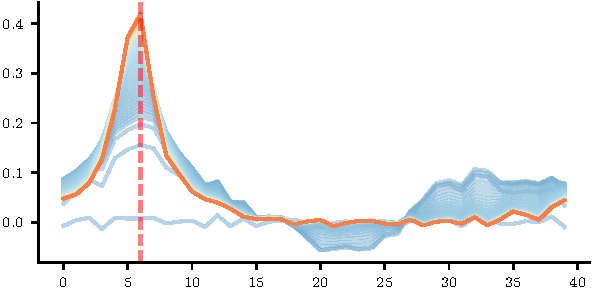
\includegraphics[height=\fieldheight]{figures/theory/rf_sim/ising_kurtosis_neurips.pdf} \\ 
      \noalign{\vskip -25pt}
      \raisebox{23pt}{
      \begin{tabular}{c}
        \small$\texttt{NLGP}(0.01)$ \\
        \hspace{4pt}
        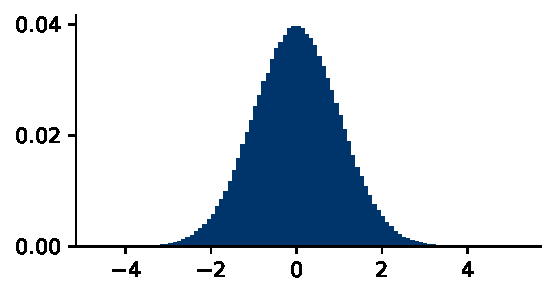
\includegraphics[height=\marginalheight]{figures/task/marginal/gaussian.pdf}
      \end{tabular}} &
      \raisebox{48pt}{\rotatebox{90}{\tiny $\varphi(a)$}} &
      \raisebox{8pt}{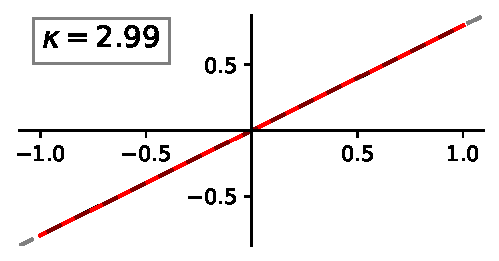
\includegraphics[height=\varphiheight]{figures/theory/varphi/gaussian.pdf}} &
      \raisebox{48pt}{\rotatebox{90}{\tiny magnitude $w_i$}} &
      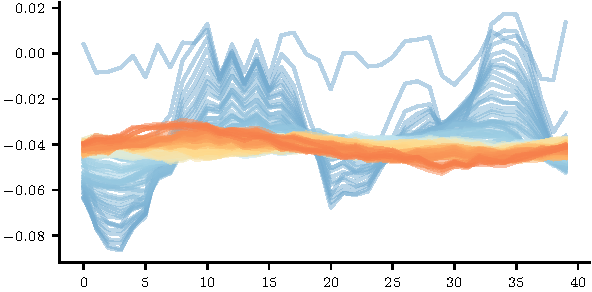
\includegraphics[height=\fieldheight]{figures/theory/rf_evol/gaussian_neurips.pdf} &
      \raisebox{48pt}{\rotatebox{90}{\tiny magnitude $w_i$}} &
      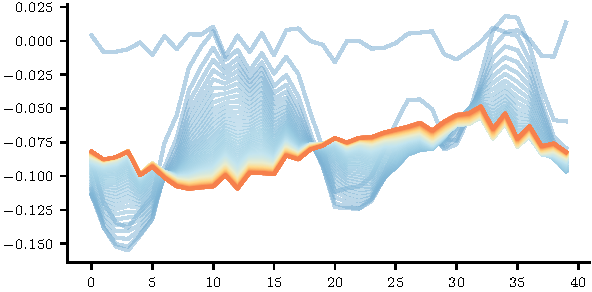
\includegraphics[height=\fieldheight]{figures/theory/rf_sim/gaussian_kurtosis_neurips.pdf} \\ 
      \noalign{\vskip -25pt}
      \raisebox{23pt}{
      \hspace{.4em}
      \begin{tabular}{c}
        \small $\texttt{Kur}(5)$ \\
        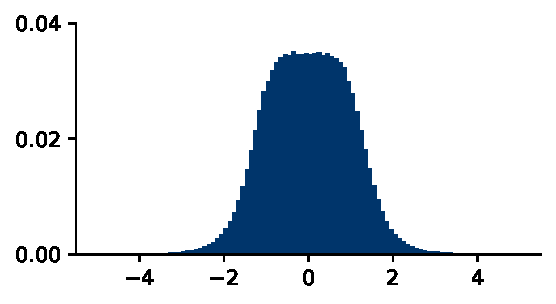
\includegraphics[height=\marginalheight]{figures/task/marginal/alg5.pdf}
      \end{tabular}} &
      \raisebox{48pt}{\rotatebox{90}{\tiny $\varphi(a)$}} &
      \raisebox{8pt}{
      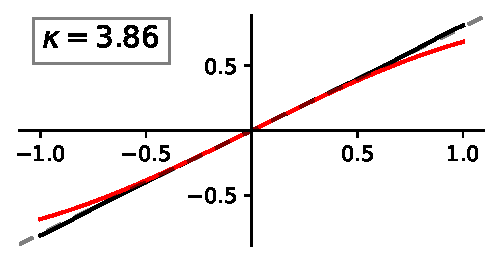
\includegraphics[height=\varphiheight]{figures/theory/varphi/alg5.pdf} 
      } &
      \raisebox{44pt}{\rotatebox{90}{\tiny magnitude $w_i$}} &
      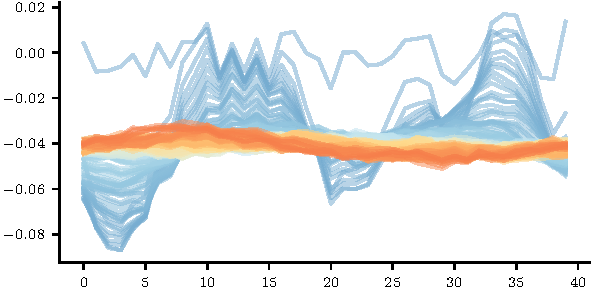
\includegraphics[height=\fieldheight]{figures/theory/rf_evol/alg5_neurips.pdf} &
      \raisebox{44pt}{\rotatebox{90}{\tiny magnitude $w_i$}} &
      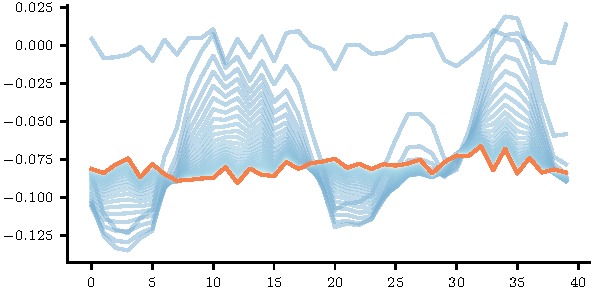
\includegraphics[height=\fieldheight]{figures/theory/rf_sim/alg5_kurtosis_neurips.pdf} \\ 
      \noalign{\vskip -40pt}
      &&
      \hspace{0pt}\tiny input value $a$ & &
      \hspace{12pt}\tiny dimension $i$ of weight $\mathbf{w}$ & &
      \hspace{12pt}\tiny dimension $i$ of weight $\mathbf{w}$ \\
    \end{tabular}
  \caption{
    From left and for the same \texttt{Ising}, \texttt{NLGP}, and \texttt{Kur} data models as in \cref{fig:task}:
    the marginals $p(X_i)$,
    the amplifier $\varphi$ defined in \cref{lem:gradient_flow} and kurtosis $\kappa$,
    and the evolution of simulated receptive fields for the single-neuron model (\labelcref{item:single-neuron-model}) trained on its data, and 
    lastly the receptive field given by numerically integrating \cref{eq:gradient_flow_early} with $\varphi$ expanded to a third-order Taylor approximation for the same data;
    training or evolution time is indicated by line color (blue for early-time; red for late-time).
    \emph{See \cref{sec:theory-validation} for exposition.}
  }
  \label{fig:theory}
\end{figure}
